\chapter{Lecture 2}

In this lecture we consider a naive example that aims to exemplify how the Euler-Lagrange equations lead us to classical BV theories.

\begin{example}
  Let $\Fcal$ be a finite-dimensional vector space encoding the naive space of fields and consider an action
  \begin{equation*}
    S: \Fcal \longrightarrow \Rbb.
  \end{equation*}
  We say that $S$ is a naive action because it might be necessary to add additional terms to $S$ to guarantee that it satisfies the CME. The solutions to the Euler-Lagrange equation are fields $f \in \Fcal$ such that ${\drm S}_f = 0$. Restricting to the case $\Fcal = M$ for some finite-dimensional manifold $M$, we say that critical points of the action form the \textbf{critical locus} of $S$
  \begin{equation*}
    \Crit (S) = \bigl\{ p \in M \bigm| \drm S_p = 0 \bigr\}.
  \end{equation*}
  Alternatively, we can characterize the critical locus of $S$ as an intersection in $T^* M$
  \begin{equation*}
    \Crit (S) = \Graph( \drm S) \cap \Graph (M)
  \end{equation*}
  where we identify $M$ with the zero section. It follows that
  \begin{equation*}
    \Ocal( \Crit (S) ) =
    \Ocal( \Graph (\drm S ) ) \otimes_{\Ocal(T^* M)} \Ocal(M).
  \end{equation*}
  We are going to consider a derived version of this construction, where the tensor product $\otimes$ is replaced by a derived tensor product $\otimes^{\Lbb}$. This raises the obvious questions:
  \begin{figure}[ht]
    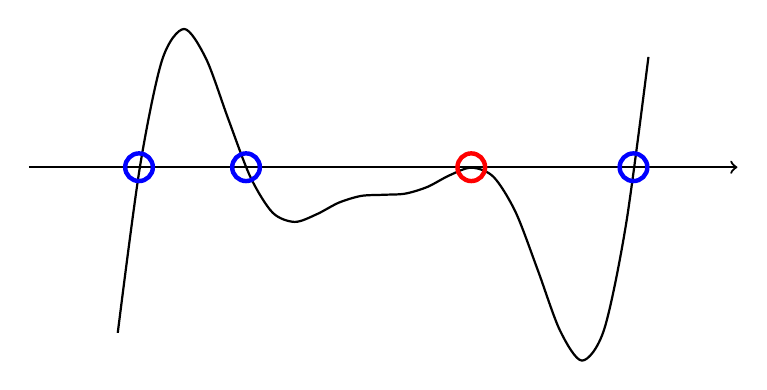
\begin{tikzpicture}
      \draw[thick, ->] (-4.5, 0) -- (4.5, 0);
      \draw[thick, domain=-3.37:3.37, smooth, variable=\x] plot ( {\x}, {.35*sin(2*deg(\x))*\x*\x-.35} );
      \draw[ultra thick, color=blue] (-3.1, 0) circle (5pt);
      \draw[ultra thick, color=blue] (-1.741, 0) circle (5pt);
      \draw[ultra thick, color=red] (1.12, 0) circle (5pt);
      \draw[ultra thick, color=blue] (3.18, 0) circle (5pt);
    \end{tikzpicture}
    \centering
    \caption{Well-behaved (in red) and badly-behaved (in red) points of an intersection.}
    \label{fig:bad_intersections}
  \end{figure}
  \begin{itemize}
    \item \textbf{Why?} This intersection might not be well behaved, in the sense that $\drm S$ and the zero section might not intersect transversally at every point, as illustrated in figure \ref{fig:bad_intersections}. The derived approach allows us to study these badly-behaved points using Serre's intersection formula.
    \item \textbf{How?} We replace $\Ocal (\Graph(\drm S)) \otimes_{\Ocal (T^*M)} \Ocal(M)$ with a dg commutative algebra $A$ such that
    \begin{equation*}
      \Hrm^0 A = \Ocal (\Graph(\drm S)) \otimes_{\Ocal (T^*M)} \Ocal(M).
    \end{equation*}
    To compute the derived tensor product $\otimes^{\Lbb}$ we need to resolve either $\Ocal(M)$ or $\Ocal(\Graph(\drm S))$ in $\Ocal(T^* M)$-modules. Let us make use of Darboux coordinates to resolve
    \begin{align*}
      \Ocal(\Graph(\drm S)) &=
      \bigslant{\Ocal(T^* M)}{ \bigl( f \vert_{\Graph(\drm S)} = 0 \bigr) } \\
                            &= \bigslant{ \Ocal( T^* M )}{ \bigl( p_{\mu} - \partial_\mu S \bigr) }.
    \end{align*}
  \end{itemize}
\end{example}

